\documentclass[language=en,11pt]{aghdpl}


\author{Aleksander Nagaj}
\shortauthor{A. Nagaj}

%\titlePL{Przygotowanie pracy dyplomowej w~systemie~\LaTeX}
\titleEN{Vision system for controlling the route of an autonomous boat using machine learning methods.}


%\shorttitlePL{Przygotowanie pracy dyplomowej w~systemie \LaTeX} % skrócona wersja tytułu jeśli jest bardzo długi
%\shorttitleEN{Preparation of a long and fascinating thesis in \LaTeX}


% Dopuszczalne wartości[1,2]:
% * "Projekt dyplomowy" - na koniec studiów I stopnia
% * "Praca dyplomowa" - na koniec studiów II stopnia
% [1] Zasady dyplomowania w roku akademickim 2020/2021 (Decyzja Dziekana WEAIiIB nr 16/2020 z dnia 9 grudnia 2020 roku)
% [2] Załącznik nr 1a) do Decyzji nr 16/2020 Dziekana Wydziału EAIiIB z dnia 09 grudnia 2020 r.
%\thesistype{Praca dyplomowa}
\thesistype{Bachelor of Science Thesis}

\supervisor{Maciej Rosół, PhD}

\degreeprogramme{Automatics and Robotics}

\date{2021}

\renewcommand{\contentsname}{Table of Contents}

\department{Department of Applied Computer Science}

\faculty{Faculty of Electrical Engineering, Automatics, Computer Science and Biomedical Engineering}

\acknowledgements{For Em}


\begin{document}
    % \setcounter{page}{1}

	\titlepages
	\RedefinePlainStyle
	
    \begin{abstract}
\setcounter{page}{3}
    Reinforcement learning methods are commonly used in various areas such as: self-driving cars, trading and finance, NLP\footnote{Natural Language Processing} and many more. Q-learning is an off-policy, model-free algorithm that found numerous applications in a training of autonomous agents. With a support of Deep Neural Network to evaluate and improve action policy, Deep Q-Learning became a powerful enough tool to teach an autonomous boat how to find a route using its vision system in an environment when it was trained. This paper gives a detailed information of how it was achieved and compares different architectures of DQN applied to solve the task given in the Thesis.
\end{abstract}


	
	\setcounter{tocdepth}{2}
	\tableofcontents
	\clearpage
	
	\chapter{Introduction}
\label{cha:introduction}

The recent development in the deep learning area has resulted in a significant increase in usage of artificial intelligence
solutions. Recommendation algorithms, voice or face recognition, type hinting - these are only examples of technologies which are
used on a everyday basis by millions. Deep Artificial Neural Networks are by far the most robust of all machine learning
algorithms capable of handling various tasks in an unprecedented manner. Thus the choice of getting hands on designing and
implementing vision system for an autonomous boat which uses their full potential.

\section{Purpose}
\label{sec:purpose}

The goal was to create a \textbf{vision system} for an autonomous agent which would be responsible for its autonomous control on a given
track limited by buoys. The system uses images retrieved from a pair of front cameras to train a \textbf{Deep Reinforcement Network}
responsible for track analysis and boat control. The entire project is held in a simulation environment where a designed algorithm is
trained on a boat model which resembles a real life counterpart. 

The expected result was a well-designed and trained Deep Reinforcement Network capable of controlling the boat within defined constraints.
Ideally the network should be tested in a real environment, however due to limited resources and time the overall performance was measured
entirely in the simulation.

\section{Real-life applications of Reinforcement Learning}
\label{sec:real-life-applications-of-deep-learning}

\subsection{Games}
\label{sub:intro-games}
RN nowadays is well-known due to algorithm which used to play different games and managed to achieve a super-human performance in some.
The DQN agent designed by \emph{Google Deep Mind} was able to play 49 different Atari 2600 games (\ref{fig:Atari2600}). However, the most
famous one is probably the \emph{AlphaGo} \cite{AlphaGO}  and \emph{AlphaGo Zero}. AlphaGo was trained on countless human games achieving
robust performance, but it was not sufficient for the researchers. They let their new agent trained from scratch - AlphaGo Zero to play with
itself and eventually beat AlphaGo 100-0. 

\begin{figure}[h]
    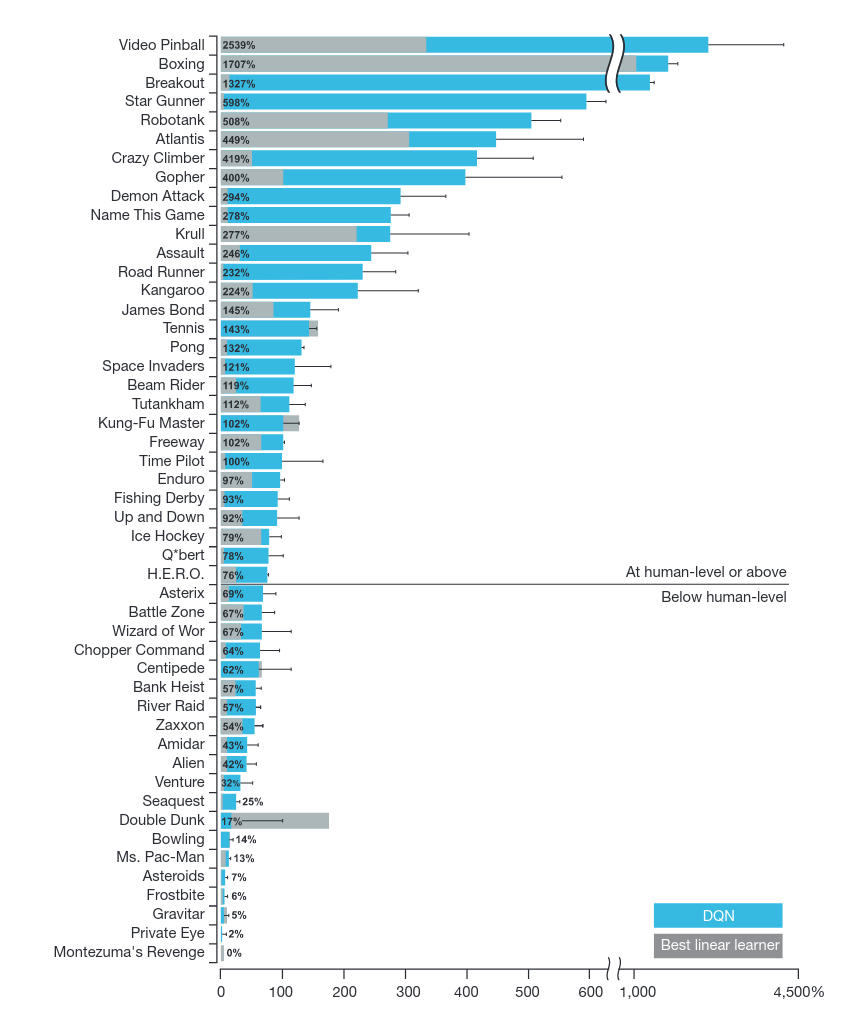
\includegraphics[width=10cm]{img/Atari2600.png}
    \centering
    \caption{Reinforcement Learning model vs human-level performance in the Atari 2600 environment \cite{DQNAtari}}
    \label{fig:Atari2600}
\end{figure}

\subsection{Robotics}
\label{sub:intro-robotics}
As stated in survey conducted by \emph{Jens Kober}, \emph{J.Andrew Bagnell}, and \emph{Jan Peters} \cite{RNSurvey}, ``\emph{Reinforcement
learning offers to a robotics a framework and set of tools for the design of sophisticated and hard-to-engineer behaviors}''. In fact, these
are most of existing ones in a real world. Instead of engineering a set of deterministic movements of a robot in a controlled environment,
identical or improved result can be achieved through training in a well-defined task which provides feedback measuring robot's performance.
Such approach enables to train robots for performing tasks in more real world environments which are not usually fully controllable.

\subsection{Personalized Recommendations}
\label{sub:intro-personalized-reccomendations}
News recommendations tends to be challenging due to the fact that most of the users easily get bored. Even if one clicks at the article,
there is a low likelihood that it will be read to the end. Therefore Click Through Rate standalone, which is used by many algorithms, is an
ineffective indicator. In order to improve the quality of recommendations and address this issue, the DQN was designed and described in
\emph{DRN: A Deep Reinforcement Learning Framework for News Recommendation} \cite{DRNNewsRecommendaiton}. This method uses multiple features
to determine what will be displayed to the user.

% 	\chapter{Przykłady elementów pracy dyplomowej}

\section{Liczba}

Pakiet \texttt{siunitx} zadba o to, by liczba została poprawnie sformatowana: \\
\begin{center}
	\num{1234567890.0987654321}
\end{center}


\section{Rysunek}

Pakiet \texttt{subcaption} pozwala na umieszczanie w podpisie rysunku odnośników do ,,podilustracji'': \\

\begin{figure}[h]
	\centering
	\begin{subfigure}{0.35\textwidth}
		\centering
		\framebox[2.0\width]{A}
		\subcaption{\label{subfigure_a}}
	\end{subfigure}
	\begin{subfigure}{0.35\textwidth}
		\centering
		\framebox[2.0\width]{B}
		\subcaption{\label{subfigure_b}}
	\end{subfigure}
	
	\caption{\label{fig:subcaption_example}Przykład użycia \texttt{\textbackslash subcaption}: \protect\subref{subfigure_a} litera A, \protect\subref{subfigure_b} litera B.}
\end{figure}

\section{Tabela}

Pakiet \texttt{threeparttable} umożliwia dodanie do tabeli adnotacji: \\

\begin{table}[h]
	\centering
	
	\begin{threeparttable}
		\caption{Przykład tabeli}
		\label{tab:table_example}
		
		\begin{tabularx}{0.6\textwidth}{C{1}}
			\toprule
			\thead{Nagłówek\tnote{a}} \\
			\midrule
			Tekst 1 \\
			Tekst 2 \\
			\bottomrule
		\end{tabularx}
		
		\begin{tablenotes}
			\footnotesize
			\item[a] Jakiś komentarz\textellipsis
		\end{tablenotes}
		
	\end{threeparttable}
\end{table}

\section{Wzory matematyczne}

Czasem zachodzi potrzeba wytłumaczenia znaczenia symboli użytych w równaniu. Można to zrobić z użyciem zdefiniowanego na potrzeby niniejszej klasy środowiska \texttt{eqwhere}.

\begin{equation}
E = mc^2
\end{equation}
gdzie
\begin{eqwhere}[2cm]
	\item[$m$] masa
	\item[$c$] prędkość światła w próżni
\end{eqwhere}

Odległość półpauzy od lewego marginesu należy dobrać pod kątem najdłuższego symbolu (bądź listy symboli) poprzez odpowiednie ustawienie parametru tego środowiska (domyślnie: 2 cm).

% 	\chapter{Testy}

\section{Test URL-a}

Wejdź na stronę \url{https://www.google.pl/} i wpisz szukane zdanie.

\clearpage

\section{Test dzielenia wdów}

Lorem ipsum dolor sit amet, ex est alia dolorem commune. Duo modo errem no. Ea harum doming atomorum mei. Consul animal malorum cu qui, sumo dicta graece an est, vim ei clita regione.

Vel eu quando doming fastidii, mei graeco indoctum an, legere theophrastus in pro. Te mei probatus eleifend interpretaris. Est no autem liber vituperatoribus, cu mea dicam constituto. Ea laudem tritani consectetuer sit, sanctus patrioque expetendis vix in. Duo id fugit adversarium signiferumque, an quot modus molestiae qui.

Ut paulo definiebas pro. Mea an quod esse. Et atomorum facilisis moderatius sit. Graeco iudicabit forensibus in vel. Eam cu lorem aeterno offendit, cu vix nulla congue posidonium. Vel lucilius evertitur vituperata no.

Mea eu graecis prodesset. Et tota eius nec. Ei etiam oratio has, vel ei homero eripuit invenire. Sed ex errem intellegebat, sea et elitr intellegat constituto. Nostro voluptua accusamus eos in, ei sale admodum has. Vim ne consetetur reformidans, ad has malis recusabo persequeris, per etiam virtute invenire in.

Te nihil eruditi eam, sit aperiam accusam mediocritatem at. Nec ne nonumy dictas disputationi, vis ridens sadipscing ex. Harum euripidis ex vix, at consetetur instructior signiferumque mel, at mei elitr honestatis. Id sit congue vituperata. Temporibus eloquentiam no eum.

Pro id esse phaedrum, nostro iudicabit eos ut. Sit ea aperiam alienum, harum audiam voluptua cu usu. Iudico invenire te vel, id suscipit disputando pri. Ut sumo expetenda mea.

Cum at idque nullam aperiam, vis ex aeque ponderum luptatum. Vix soluta graeco dissentiet ut, ut est reque periculis similique, ut dicta dicant repudiare sea. Ne dolor legendos signiferumque ius, at eirmod convenire qui. Suas numquam conceptam mei ex. Autem homero eos et, sea dicta alienum iudicabit ut.

Ea duo consulatu vulputate, id elit perpetua cum. His ei aeque saepe audiam. Prompta laoreet facilisi ne sed, per hinc consetetur te, oratio fuisset ullamcorper mel at. Quis suscipiantur ne nec, agam efficiendi usu in.

Vis eu iuvaret singulis appellantur, usu ex saepe omittantur. Sed possit mnesarchum at, usu illum choro oratio in, et debet dolor vix. Mel aperiri suscipiantur ne, te per illum fuisset, lorem pericula mei ad. Pri id tale lucilius dissentiet, id sea sonet expetenda. Agam sensibus persequeris sed no, eum at tamquam sanctus.

Omnis exerci soleat ut vis. Rebum vidisse sea ex. Ius animal gubergren efficiantur ad, mollis probatus nec ut. Meis platonem ex vel, ut qui tale tritani equidem. Vide meis fuisset mel at, nam an assum delenit gubergren. No illum reprimique vim, te augue nullam per, ludus dicant suscipiantur ne sed.

An pri mediocrem deseruisse, ad sumo audire dissentiet sit. Sit ea civibus lobortis. Etiam ceteros commune ei vis. Pro ei equidem vivendo. Quo ne prima periculis omittantur, ex rebum veritus sit, ei dolor maiestatis mea.

\subsection{Lorem ipsum}

Et mel munere quodsi sapientem. Essent legimus ne pro. Est ornatus definiebas et. No habemus docendi ius, purto sapientem mei at. Tamquam vivendo necessitatibus has at, no habemus praesent nec. No quo modus iudicabit scriptorem. Modus intellegebat ea vim. Cu ius lorem regione offendit, ne accusata sensibus vituperatoribus quo. Sit ut iuvaret indoctum. Ut mea sale justo. Sapientem definitionem ius eu, at sea quem doming. Facete conclusionemque ut nec, vix at duis eius. Eos quot consequuntur et, ornatus liberavisse ne mei.

Per an dicam commodo tractatos, usu in timeam numquam tacimates. Case delectus eu sea, usu audiam eleifend tincidunt id, nec at decore discere mentitum. Ut elit veri eloquentiam his, ceteros tractatos ea has. Duo impetus scribentur et, eu quo errem everti, ad recusabo consulatu ius. Fastidii comprehensam pri ea, ex duo augue quando denique. Eos aeterno deserunt sententiae cu, ius quas tation patrioque ex.

Id autem scripta explicari nec, congue quidam possit te sit. Et usu ipsum bonorum graecis, ferri verear deterruisset eum cu. Purto porro accommodare cu vim. Cum ei tritani pertinacia voluptaria.
	
	% itd.
	% \appendix
	% \include{dodatekA}
	% \include{dodatekB}
	% itd.
	
	\printbibliography

\end{document}
